\documentclass[12pt, a4paper]{article}
\usepackage[T2A]{fontenc}
\usepackage{amsfonts}
\usepackage{amsmath}
\usepackage{mathabx}
\usepackage{graphicx}
\usepackage{hyperref}
\usepackage{listings}
\usepackage{color}
\usepackage[margin=0.25in]{geometry}
\usepackage{pgfplots}
\pgfplotsset{width=10cm,compat=1.9}
\usepackage{nicefrac}
\graphicspath{../Images}
\usepackage{tikz}
\usepackage{cancel}

\definecolor{dkgreen}{rgb}{0,0.6,0}
\definecolor{gray}{rgb}{0.5,0.5,0.5}
\definecolor{mauve}{rgb}{0.58,0,0.82}


\lstset{frame=tb,
language=C++,
  aboveskip=3mm,
  belowskip=3mm,
  showstringspaces=false,
  columns=flexible,
  basicstyle={\small\ttfamily},
  numbers=none,
  numberstyle=\tiny\color{gray},
  keywordstyle=\color{blue},
  commentstyle=\color{dkgreen},
  stringstyle=\color{mauve},
  breaklines=true,
  breakatwhitespace=true,
  tabsize=3
  }
  
  \title{Алгоритмы и структуры данных 1 модуль.}
  \author{Андрей Тищенко \href{https://t.me/AndrewTGk}{@AndrewTGk}}
  \date{2024/2025}
  \renewcommand*\contentsname{Контент}
  
  \begin{document}
  \maketitle
  \tableofcontents
    \begin{center}
        \textbf{Лекция 3 сентября.}
    \end{center}
    \section*{\text{Выставление оценок}}
    $\text{Накоп} = 0.25\text{Коллок} + 0.25\text{КР} + 0.4\text{ДЗ} + 0.1\text{РС}$.\\
    Коллоквиум между 1 и 2 модулем. После коллока 
    письменная контрольная работа (примерно в конце 
    второго модуля).\\
    ДЗ --- контест.\\ 
    РС --- работа на семинаре.\\
    $\text{Итог} = \text{Накоп}\ \text{или}\ 0.5\text{Накоп} + 0.5\text{Экз}$ (экзамен можно не сдавать).\\
    В первом случае накоп округляется, во втором --- нет.
    \section{Структуры данных}
    $\textit{Абстракный тип данных}$ --- определяется набор операций, 
    но умалчивается реализация.\\
    $\textit{Структура данных}$ --- реализация абстаркного типа данных.
    \subsection{Линейные структуры данных}
    \subsubsection*{Массив}
    \begin{lstlisting}
        int a[20];
        array<int, 20> a;
        vector<int> a(20); // O(1) amortized 
        // amortized means average O(1), but O(n) is possible
    \end{lstlisting}
    \subsection{Список}
        \subsubsection*{Виды списков}
        \begin{enumerate}
            \item Односвязный (храним указатель на начало и конец, указатель на следующий элемент).
            \item Двусвязный (аналогично односвязному, но также указатель на предыдущий).
        \end{enumerate}
    \subsection{Стек}
        Свойства: LIFO (last in, first out)
        \subsubsection*{Реализация}
        Массив: простая реализация, так как переполнение невозможно.\\
        Список: возвращаем head, добавление в head (список двусвязный).\\
        deque: добавление и взятие элементов из начала или конца (покрывает функционал).
        \subsubsection*{Виды стеков}
        \begin{enumerate}
            \item Стек с минимумом (дополнительный стек, который хранит минимумы на префиксах).
        \end{enumerate}
    \subsection{Очередь}
        Свойства: FIFO (first in, first out)
        \subsubsection*{Реализация}
        Массив: кладём элементы по очереди, после переполнения массива мы должны класть элементы в начало (храним указатель на начало и конец очереди).\\
        Список: Возвращаем tail, добавление в head (список двусвязный).\\
        deque: добавление и взятие элементов из начала или конца (покрывает функционал).\\
        Два стека: кладём элементы в первый стек, если нужно взять элемент, то берём из второго стека. Если второй стек пустой, перекладываем все элементы во второй стек. Амортизированное $O (1)$.
    \subsection{Устройство вектора}
        Выделяет какое-то базовое количество памяти по умолчанию. Хранится указатель на начало, конец используемой пользователем памяти и конец аллоцированной памяти.\\
        Когда конец используемой пользователем памяти совпадает с концом аллоцированной памяти, аллоцируется кусок памяти 
        в $1.5$ или $2$ (зависит от реализации) раза больше. Получается, что при выполнении $n$ пушбеков, вектор перезапишет себя 
        не более $\log n$ раз. Всего будет переписано не более $1 + \cdots + \frac{n}{2} + n \approx 2n = O(n)$.
    \section{Метод потенциалов анализа сложности}
        $\varphi$ --- функция подсчёта потенциала (зависит от параметров структуры данных).\\
        $\varphi_0\rightarrow \varphi_1 \rightarrow \varphi_2 \rightarrow\dots\rightarrow  \varphi_n$\\
        Определение: амортизированное время работы:\[a_i = t_i + \Delta \varphi,\ \Delta \varphi = \varphi_{i + 1} - \varphi_i\]
        $\sum a_i = \sum t_i + (\varphi_n - \varphi_0)\Rightarrow \frac{\sum t_i}{n} = \frac{\varphi_0 - \varphi_n}{n} + \frac{\sum a_i}{n} \leq \frac{\varphi_0 - \varphi_n}{n} + \max(a_i)$\\
        $\varphi_i = 2n_1$\\
        push: $t_i = 1,\ a_i = 1 + 2 = 3$\\
        pop: $t_i = 1\text{ или } t_i = 2n_1 + 1,\ a_i = 1\text{ или } a_i = 2n_1 + 1 + (0 - 2n_1) = 1$\\
        Значит $\max(a_i) \leq 3$, при этом $\frac{\varphi_0 - \varphi_n}{n} \leq 0$, то есть амортизированное время работы:
        \[\frac{\sum t_i}{n} \leq 3\]
    \begin{center}
        \textbf{Лекция 10 сентября.}
    \end{center}
    \section{Символы Ландау}
    Оценка сверху:
    \[f(x) = O\big(g(x)\big)\Leftrightarrow \exists C > 0\ \exists x_0 \geq 0\ \forall x\geq x_0:\ |f(x)|\leq C|g(x)|\]
    Оценка снизу:
    \[f(x) = o\big(g(x)\big)\Leftrightarrow \forall \varepsilon > 0\ \exists x_0\ \forall x\geq x_0:\ |f(x)| \leq \varepsilon|g(x)|\]
    Равенство функций:
    \[f(x) = \Theta\big(g(x)\big)\Leftrightarrow \exists 0 < C_1 < C_2,\ \exists x_0\ \forall x \geq x_0:\ C_1|g(x)| \leq |f(x)| \leq C_2|g(x)|\]
    \underline{Примеры:}
    \begin{enumerate}
        \item $3n + 5\sqrt{n} = O(n)$
        \item $n = O(n^2)$. Оценка грубая, но правильная, потому что $n \leq n^2$. Лучше было бы понять, что $n = O(n)$
        \item $n! = O(n^n)$
        \item $\log n^2 = O(\log n)$
        \item Пусть мы в задаче ввели параметр k, при этом оптимально, чтобы выполнялось соотношение $k\log k = n$. Как можно оценить $k$?\\
        $k = O(?)$, обсудим на семинаре.
    \end{enumerate}
    \subsection*{Задача}
    Найти асимптотику сортировки слиянием.\par
    Пусть $T(n)$ --- время, используемое для сортировки массива длины $n$.\\
    Зная принцип работы этой сортировки можно сказать, что
    \[T(n) = 2\cdot T\left(\frac{n}{2}\right) + O(n)\]
    \underline{Сформулируем \textbf{Мастер теорему}}\label{sec:MasterTh}
    \[T(n) = \begin{cases}
        aT\left(\frac{n}{b}\right) + O(n^c),\ a\in \mathbb{N},\ b\in \mathbb{R},\ b>1,\ c\in \mathbb{R},\ c\geq 0\\
        O(1),\ n\leq n_0
    \end{cases}\]
    Разберём три случая:
    \begin{enumerate}
        \item $c > \log_b a:\ T(n) = O(n^c)$
        \item $c = \log_b a:\ T(n) = O(n^c\log n)$
        \item $c < \log_b a:\ T(n) = O(n^{\log_b a})$
    \end{enumerate}
    % \includegraphics{AaDS_Tree.png}
    На $i$-ом слое: $a^i\left(\frac{n}{b^i}\right)^c$\\
    Листья (слой $\log_b n$): $a^{\log_b n}$ задач, сложность каждой равна 1\\
    $T(n) \leq \displaystyle \sum_{i = 0}^{\log_b n} O \left(a^i\left( \frac{n}{b^i} \right)^c\right) = O\left( \sum_{i = 0}^{\log_b n} a^i \left( \frac{n}{b^i} \right)^c \right) = O\left( n^c \sum_{i = 0}^{\log_b n} \left( \frac{a}{b^c}  \right)^i \right)$\\
    Положим $q = \frac{a}{b^c}$, тогда:\\
    $q < 1\Leftrightarrow a < b^c\Leftrightarrow c > \log_b a,\ \displaystyle O\left(n^c \sum_{i = 0}^{\log_n b} q^i\right) = O\left(n^c \frac{1}{1 - q}\right) = O\left(n^c\right)$\\
    $q = 1\Leftrightarrow O(n^c \log_b n)$\\
    $q > 1$:\\
    Докажем \textit{лемму}:
    \[\forall q > 1:\ 1 + q + \cdots + q^n = O(q^n)\]
    $\frac{q^{n + 1} - 1}{q - 1} < \frac{q^{n + 1}}{q - 1} = \frac{q}{q - 1}q^n = O(q^n)$\\
    Тогда для $q > 1$: $O\left(n^c \left( \frac{a}{b^c} \right)^{\log_b n} \right) = O\left( n^c \frac{a^{\log_b n}}{b^{c\log_b n}} \right) = O\left( n^c \frac{a^{\log_b n}}{n^c} \right) =\\
    = O\left( a^{\log_b n} \right) = O\left( n^{\log_b a} \right)$
    \subsection*{Примеры}
    Сортировка слиянием:\\
    $T(n) = 2T(\frac{n}{2}) + O(n^1)\Rightarrow\\
    \Rightarrow a = 2,\ b = 2,\ c = 1\Rightarrow \log_b a = c \wedge T(n) = O(n^c\log n) = O(n\log n)$\\
    Бинарный поиск:\\
    $T(n) = T(\frac{n}{2}) + O(1)\Rightarrow\\
    \Rightarrow a = 1,\ b = 2,\ c = 0\Rightarrow \log_b a = c\Rightarrow T(n) = O(n^c\log n) = O(\log n)$\\
    Обход полного двоичного дерева с $n$ вершинами:\\
    $T(n) = 2T(\frac{n}{2}) + O(1)\Rightarrow\\
    \Rightarrow a = b = 2,\ c = 0\Rightarrow \log_2 2 > 0\Rightarrow T(n) = O\left(n^{\log_b a}\right) = O(n^1) = O(n)$
    \begin{center}
        Лекция 17 сентября
    \end{center}
    \section{Алгоритмы быстрого умножения}
    \subsection{Алгортим Карацуба}
    \hspace{0.5cm}Придумали в 1960 году. Этот алгоритм мотивировал людей искать более быстрые способы решения известных задач. (На коллоквиуме может пригодиться базовое знание алгоритма Фурье).
    \begin{center}
        \underline{\textbf{brute}}\footnote[1]{Далее так будут называться решения в лоб или переборные решения}
    \end{center}
    $A(x) = a_0 + a_1 x + \cdots + a_{n - 1}x^{n - 1}$. Будем называть это многочленом с $n$ коэффициентами ($(n)$-член в дальнейшем).\\
    $B(x) = b_0 + b_1 x + \cdots + b_{m - 1}b^m$ - $(m)$-член\\
    $C(x) = A(x)\cdot B(x) = c_0 + c_1 x + \cdots + c_{n + m - 2}x^{n + m - 2}$ - $(n + m - 1)$-член\\
    $c_k = \displaystyle \sum_{i = 0}^{k} a_i\cdot b_{k - i}$ - k-ый коэффициент в $C(x)$\\
    Такое решение имеет асимптотику $O(n\cdot m)$. Мы будем писать алгоритм для перемножения многочленов одинаковых степеней, поэтому асимптотика будет $O\big(\max(n,\ m)^2\big)$, где $\max(n,\ m)$ - степень двойки.\\
    $A(x) = a_0 + a_1 x + \cdots + a_{n - 1}x^{n - 1} =\\
    =\big(\underset{A_0(x)}{\underbrace{a_0 + a_1 + \dots + a_{\frac{n}{2} - 1}x^{\frac{n}{2} - 1}}}\big) + \big( \underset{A_1(x)}{\underbrace{a_{\frac{n}{2}} + a_{\frac{n}{2} + 1}x^{1} + \dots + a_{n - 1} x^{\frac{n}{2} - 1}}} \big)x^{\frac{n}{2}}$\\
    Аналогично разбиваем $B(x) = B_0(x) + B_1(x)x^{\frac{n}{2}}$, тогда:\\
    $A(x)\cdot B(x) = (A_0 + A_1 x^{\frac{n}{2}})(B_0 + B_1 x^{\frac{n}{2}}) = A_0 B_0 + (A_1 B_0 + A_0 B_1)x^{\frac{n}{2}} + A_1 B_1 x^n$\\
    Однако если это тупо перемножить, то мы ничего не выиграем:\\
    $T(n) = 4T\left(\frac{n}{2}\right) + O(n)$. По мастер теореме $a = 4,\ b = 2,\ c = 1\Rightarrow\\
    \Rightarrow 1 < \log_2 4 = 2\Rightarrow T(n) = O(n^2)$\\
    Методом подстановки получаем такую же асимптотику (опускаем O(n), так как здесь оно не сильно влияет).\\
    $T(n) = 4T(\frac{n}{2}) = 4^2 T(\frac{n}{2^2}) = \dots = 4^kT(\frac{n}{2^k})$.\\
    В какой-то момент $2^k = n\Rightarrow 4^k = n^2\Rightarrow T(n) = n^2T(1) = n^2$\\
    Идея Карацубы заключается в выполнении трёх умножений вместо четырёх.\\
    Сделаем два умножения: $A_0 B_0,\ A_1 B_1$, далее алгебраические фокусы:\\
    Делаем умножение $(A_0 + A_1)(B_0 + B_1) = A_0 B_0 + A_1 B_1 + A_0 B_1 + A_1 B_0$, тогда:
    $(A_1B_0 + A_0B_1) = (A_0 + A_1)(B_0 + B_1) - A_0 B_0 - A_1 B_1$.\\
    Этот метод работает быстрее, так как сложение и вычитание мы выполняем за линию, то есть за 2 сложения и два вычитания (4 линии) экономим одно умножение (квадрат).\\
    Теперь $T(n) = 3T\left(\frac{n}{2}\right) + O(n)\overset{\text{M Th}}{\Longrightarrow}\footnotetext{\text{M Th = \hyperref[sec:MasterTh]{Мастер Теорема}}} 1 < \log_2 3\Rightarrow T(n) = O(n^{\log_2 3})$\\
    Проверим методом подстановки: $n = 2^k:\ O(3^k) = O(3^{\log_2 n}) = O(n^{\log_2 3})$\\

    \subsection{Алгоритм Штрассена}
    Придуман в 1969 для умножения матриц.\\
    Математически: $C = \underset{n\times n} A \cdot \underset{n\times n}{B}$, асимпотика $O(n^3)$\\
    $C_{i\, j} = \displaystyle \sum_{k = 0}^{n - 1} a_{i\, k}\cdot b_{k\, j}$.\\
    Алгоритм заключается в следующем преобразовании:
    \[\begin{pmatrix}
        a_{1\, 1} & \vdots & a_{1\, 2}\\
        \dots & . & \dots \\
        a_{2\, 1} & \vdots & a_{2\, 2}
    \end{pmatrix}\cdot \begin{pmatrix}
        b_{1\, 1} & \vdots & b_{1\, 2}\\
        \dots & . & \dots \\
        b_{2\, 1} & \vdots & b_{2\, 2}
    \end{pmatrix} = \begin{pmatrix}
        a_{1\, 1}b_{1\, 1} + a_{1\, 2}b_{2\, 1} & \vdots & a_{1\, 1}b_{1\, 2} + a_{1\, 2}b_{2\, 2}\\
        \dots & . & \dots \\
        a_{2\, 1}b_{1\, 1} + a_{2\, 2}b_{2\, 1} & \vdots & a_{2\, 1}b_{1\, 2} + a_{2\, 2}b_{2\,2}
    \end{pmatrix}\]
    $d = (a_{1\, 1} + a_{2\, 2})(b_{1\, 1} + b_{2\, 2})\\
    d_1 = (a_{1\, 2} - a_{2\, 2})(b_{2\, 1} + b_{2\, 2})\\
    d_2 = (a_{2\, 1} - a_{1\, 1})(b_{1\, 1} + b_{1\, 2})\\
    h_1 = (a_{1\, 1} + a_{1\, 2})b_{2\, 2}\\
    h_2 = (a_{2\, 1} + a_{2\, 2})b_{1\, 1}\\
    v_1 = a_{2\, 2}(b_{2\, 1} - b_{1\, 1})\\
    v_2 = a_{1\, 1}(b_{1\, 2} - b_{2\, 2})$\\
    $T(n) = 7T\left(\frac{n}{2}\right) + O(n^2)\Rightarrow T(n) = O(n^{\log_2 7\approx 2,81})$\\
    \addcontentsline{toc}{subsubsection}{Улучшения}
    \subsubsection*{Алгоритм Копперсмита-Виноградова (1990)}
    Работает за $O(n^{2,3755})$. Является улучшением алгоритма Штрассена.\\
    \subsubsection*{Алгоритм Алмана Вильямса (2020)}
    За $O(n^{2,3728})$.\\
    \addcontentsline{toc}{subsubsection}{Гипотеза Штрассена}
    \subsubsection*{\underline{Гипотеза Штрассена}}
    $\forall \varepsilon > 0\ \exists \text{ алгоритм}\ \exists N\ \forall n \geq N:\ O(n^{2 + \varepsilon})$
    \subsection{Быстрые преобразования Фурье}
    $O(n\log n)$. Переменожаем n-члены, где $n$ - степень двойки.\\
    Храним многочлен в виде $n$ его специально подобранных точек (по ним можно восстановить коэффициенты). На коллоквиуме понадобится знать 
    основную идею работу и асимптотику.
    \section{Вероятностные алгоритмы}
    Для детерминированных алгоритмов есть понятия:\\
    \underline{Сложность} --- количество операций на данных размера n.\\
    \underline{Сложность в среднем} --- математическое ожидание количества действий.
    \underline{Вероятностный алгоритм} --- использует генератор случайных чисел.
    Могут быть алгоритмы:
    \begin{itemize}
        \item Работающие без ошибок
        \item С односторонней ошибкой
        \item С двусторонней ошибкой
    \end{itemize}
    \underline{Ожидаемое время} --- математиеческое ожидание времени работы (на \underline{\underline{одном}} наборе данных)\\
    \underline{Ожидаемая сложность} --- максимальное время работы на данных размера $n$.\\
    \subsection*{Поиск k-ой порядковой статистики}
    Выбираем опорный элемент $i$. Пусть меньше него в массиве $m - 1$ элемент, а больше него $n - m$ элементов.\\
    Тогда $E\big(T(n)\big) =\displaystyle \sum_{m = 1}^{n}P(m) E\Big(T\big(\max(m - 1,\ n - m)\big)\Big) + O(n) =\\
    = \sum_{m = \frac{n}{2}}^{n}\frac{1}{n} 2 T(m) + O(n) = \frac{2}{n}\sum_{m = \frac{n}{2}}^{n - 1} E\big(T(n)\big) + O(n) =\\
    = \frac{2}{n}\big(O(\frac{n}{2}) + O(n - 1)\big) + O(n) = \frac{2}{n}O(\frac{3n^2}{8}) + O(n) = O(\frac{3}{4}n) + O(n) = O(n)$\\
    Получаем $E\big(T(n)\big) = O(n)$ по индукции.\\
    \begin{center}
        Детерминированный поиск медианы.
    \end{center}
    Делим массив на группы по 5 чисел, сортируем их за 7 сравнений (или за 10 действий пузырьком), тратим на это $7\frac{n}{5}$ действий.\\
    Получаем $\frac{n}{5}$ медиан: $m_1,\dots,\ m_{\frac{n}{5}}$ рекуррентно ищем медиану в них, пусть это $m_s$. Тогда:\\
    $\frac{n}{10}\text{медиан} \leq m_s \leq \frac{n}{10}\text{медиан}$. Для каждой медианы слева справедливо, что есть два числа, меньше неё. Справа --- есть два числа больше неё. Так как это были медианы в пятёрках чисел.\\
    $T(n) = T\left(\frac{7n}{10}\right) + T(\frac{n}{5}) + O(n) \leq T\left(\frac{7n}{10}\right) + T(\frac{n}{5}) + C(n)\Rightarrow\\
    \Rightarrow T(n)\leq 10C\cdot n\Rightarrow T(n) = O(n)$
    \addcontentsline{toc}{subsection}{Алгоритм Фреймвальдса}
    \subsection*{Алгоритм Фреймвальдса}
    Умножаем $A\cdot B = C,\quad n\times n$\\
    $v = \left(\begin{matrix}
        0\\
        1
    \end{matrix},\ \begin{matrix}
        0\\
        1
    \end{matrix},\dots \begin{matrix}
        0\\
        1
    \end{matrix} \right) $ случайные числа 0 или 1\\
    $A\cdot B\cdot v = C\cdot v\Rightarrow O(n^2)$\\
    Если получили равенство, то вероятность $A\cdot B \neq C$: $P_{\text{неудачи}} \leq \frac{1}{2}$
    \subsubsection*{Доказательство}
    Положим $D = AB - C = \begin{pmatrix}
        d_{1\, 1} & \dots & d_{1\, n}\\
        \dots & \dots & \dots\\
        d_{n\, 1} & \dots & d_{n\, n}
    \end{pmatrix},$ без ограничения общности в нём $d_{1\, 1} \neq 0$\\
    Тогда при домножении матрицы $D$ на вектор $v$. Вероятность наличия на нужной позиции в $v$ нуля есть $\frac{1}{2}$ (так как вектор состоит из 0 и 1).
    $Dv = \begin{pmatrix}
        d_{1\, 1} v_1 + (d_{1\, 2} v_2 + \dots + d_{1\, n} v_n)\\
        \dots\\
        \dots
    \end{pmatrix}\\
    \left( \frac{m}{2^n} \right)^k \leq \left( \frac{1}{2} \right)^k$
    \addcontentsline{toc}{subsection}{Лемма Шварца-Зиппеля}
    \subsection*{Лемма Шварца-Зиппеля}
    $f(x_1,\dots,\ x_k)$ --- многочлен степени $n$ от $k$ переменных.\\
    Возьмём точку $Y = (y_1,\dots,\ y_k)$ равновероятно из множества $S$ (множество значений).\\
    $P\big(f(y_1,\dots,\ y_k)\big) \leq \frac{n}{|S|}$\\
    Дерандомизация: положим $k$ = 1 и смотрим $n + 1$ точку.
    \begin{center}
        Лекция 1 октября.
    \end{center}
    \addcontentsline{toc}{subsection}{Быстрая сортировка}
    \subsection*{Быстрая сортировка}
    Пусть изначальный массив $a = \{a_1,\dots,\ a_b\}$\\
    Хотим произвести операцию $a\rightsquigarrow b = \{b_1,\dots,\ b_n\}$, где $b_1\leq\dots\leq b_n$.\\
    $E\big(T(n)\big) = \displaystyle E\left( \sum_{i = 0}^{n - 1}\sum_{j = i + 1}^{n} \delta_{i\, j} \right) = \sum_{i = 0}^{n - 1}\sum_{j = i + 1}^{n} E(\delta_{i\, j}) = \sum_{i = 0}^{n - 1}\sum_{j = i + 1}^{n} P(b_i \text{ сравнивается с } b_j)$\\
    $\delta_{i\, j} = \operatorname{bool}(b_i \text{ сравним с } b_j)$\\
    Рассмотрим массив $b$, посмотрим на $b_i$ и $b_j$:\\
    \[b_1\leq b_2\leq\dots \leq \overset{j - i + 1\ \text{элемент}}{\overbrace{b_i \leq \dots \leq b_j}}\leq \dots \leq b_n\]
    Нас интересует выбор элемента из этих $j - i + 1$. Если выберем что-то между, то интересующие нас два сравниваться не будут. Если выберем один из них, то придётся сравнивать.\\
    Вероятность выбора $b_i$ или $b_j$ из $j - i + 1$ равна $\frac{2}{j - i + 1}$\\
    Тогда $E\big( T(n) \big) = \displaystyle \sum_{i = 0}^{n - 1}\sum_{j = i - 1}^{n} \frac{2}{j - i + 1} = \sum_{i = 0}^{n - 1}\sum_{k = 1}^{n - i} \frac{2}{k + 1} = \sum_{i = 0}^{n - 1}O(\log n) = O(n\log n)$
    \addcontentsline{toc}{subsection}{SkipList}
    \subsection*{SkipList}
    Является стурктурой данных, придумал \href{https://en.wikipedia.org/wiki/William_Pugh_(computer_scientist)}{William Pugh} в 1989 году.\\
    Сначала представлял собой отсортированный список, первым элементом которого является $-\infty$, имеющий большое количество указателей в вершинах (у каждого второго был указатель для прыжка на 2, у каждого 4 --- на 4 и т.д.), но возникали проблемы с удалением.\\
    Появилась новая идея. Создать список ``второго уровня'', в который с вероятностью $\frac{1}{2}$ попадают элементы изначального списка ($-\infty$ и элемент сразу после неё попадает во все уровни).\\
    У каждого элемента получившегося списка есть указатель на следующий элемент и на его копию на более низком уровне.\\
    По получившемуся списку мы проходим в два раза быстрее, поэтому мы создаём аналогичный список, базируясь на втором уровне, продолжая это до тех пор, пока размер получившегося уровня не станет меньше либо равен 2.\\
    В среднем на каждом уровне количество элементов уменьшается вдвое.
    \subsubsection*{Поиск}
    В такой структуре данных поиск можно осуществлять бинарным поиском.
    \subsubsection*{Удаление}
    В случае удаления элемента, он должен удаляться во всех уровнях. Пусть мы удаляем элемент $x$, тогда при рекурентном бинарном поиске этого элемента мы получим указатели $l < x \leq r$  для каждого уровня. Если $r$ совпадает с $x$, то $r$ удаляется как в обычно списке, иначе на этом и на всех уровнях выше $x$ уже не будет, удаление завершено. Перебалансировку мы не производим, так как вероятность существенно уменьшить количество уровней крайне мала.
    \subsubsection*{Вставка}
    Ищем позицию для вставки, после чего вставляем его на более высокий уровень с вероятностью $\frac{1}{2}$. В результате этой операции количество уровней могло увеличиться (в теории оно могло увеличиться более чем на 1, но на практике более чем на 1 уровень увеличивать смысла нет).
    \subsubsection*{Оценка количества уровней}
    $P(\text{есть i-й уровень}) = 1 - \left( 1 - \frac{1}{2^i} \right)^n \leq 1 - (1 - \frac{n}{2^i}) = \frac{n}{2^i}\\
    i = 4\log_2 n\quad P(i) \leq \frac{n}{4\log_2 n} = \frac{n}{n^4} = \frac{1}{n^3}$, то есть вероятность сильно превзойти $\log_2 n$ очень мала. 
    \subsubsection*{Оценка оптимальной вероятности повышения}
    Пусть $p \neq \frac{1}{2}$, тогда $n,\ pn,\ p^2 n,\dots,\ 1$ --- размеры слоёв.\\
    $\log_{\frac{1}{p}} n$ --- количество слоёв.\\
    Асимптотика: $O\left(\frac{1}{p}\log_\frac{1}{p} n\right)$
    \addcontentsline{toc}{subsection}{Алгоритм имитации отжига}
    \subsection*{Алгоритм имитации отжига}
    Введём \underline{функционал качества} $Q_0\rightsquigarrow Q_1\rightsquigarrow Q_2\rightsquigarrow\dots$.\\
    Это некая функция, которую стоит минимизировать. Программа производит случайные изменения, после чего смотрит на изменение функционала.\\
    $Q_{i + 1} < Q_i\Rightarrow$ делаем изменение.
    $Q_{i + 1} > Q_{i}\Rightarrow$ делаем изменение с вероятностью $p = e^{-\frac{Q_{i + 1} - Q_i}{T_i}}$\\
    $T_i$ - некая убывающая функция (гипербола, линейная, что лучше подходит).

    \begin{center}
        Лекция 8 октября.
    \end{center}
    \section{Численное интегрирование}
    Подсчёт площади функции $f(x)$ на отрезке $[a,\ b]$.
    \addcontentsline{toc}{subsection}{Метод Монте-Карло}
    \subsection*{Метод Монте-Карло}
    Составляем описанный прямоугольник для этой функции. Случайным образом помещаем в него точки. Далее составяем пропорцию: площадь прямоугольника отностися к площади фигуры так же как количество помещённых точек относится к количеству точек, попавших в нашу фигуру.\\
    \addcontentsline{toc}{subsection}{Метод прямоугольников}
    \subsection*{Метод прямоугольников}
    Поделим отрезок $[a,\ b]$ на $n$ равных частей, далее скадываем площади $S$ получившихся трапеций.
    $a = x_0 < x_1 <\dots < x_n = b,\ h = \frac{b - a}{n},\\
    \begin{cases}
        S = h\cdot f(x_i)\text{ --- метод левых прямоугольников}\\
        S = h\cdot f(x_{i + 1})\text{ --- метод правых прямоугольников}\\
        S = h\cdot f\left(\frac{x_i + x_{i + 1}}{2}\right)\text{ --- метод центральных прямоугольников}
    \end{cases} $
    \addcontentsline{toc}{subsection}{Метод трапеций}
    \subsection*{Метод трапеций}
    Разбиваем аналогично, но площадь считаем по формуле\\
    $S = \frac{h}{s}\big(f(x_i) + f(x_{i + 1})\big)$

    \addcontentsline{toc}{subsection}{Формула Симпсона}
    \subsection*{Формула Симпсона}
    Разбиваем на равные отрезки, для каждого отрезка считаем:\\
    $S = \frac{h}{6}\Big( f(x_i) + 4f\left( \frac{x_i + x_{i + 1}}{2} \right) + f(x_{i + 1}) \Big)$
    \subsection*{Подсчёт площади круга}
    Пусть окружность задаётся уравнением $(x - 1)^2 + (y - 5)^2 = 9$\\
    Разобьём окружность на полуокружности: $y = 5 \pm \sqrt{9 - (x - 1)^2}$\\
    Пусть $f_1(x) = 5 + \sqrt{9 - (x - 1)^2},\ f_2(x) = 5 - \sqrt{9 - (x - 1)^2}$\\
    Тогда искомая площадь: $\displaystyle \int_{-2}^4 f_1(x) - f_2(x)\, dx$\\
    Для подсчёта этих интегралов стоит написать рекурретную функцию. Она должна на отрезках с недостаточной точностью добавлять новые точки, пока точность нас не устроит. (так называемая переменная сетка).
    \subsection*{Сетка переменной плотности}
    Рассматриваем полученную на отрезке площадь, обозначим её $S_1$. Всё-таки поделим пополам и посчитаем полученную площадь, обозначим её $S_2$. Выбираем необходимую точность $\varepsilon$, если выполняется\\
    $|S_1 - S_2| < \varepsilon$, то точку мы оставляем.
    \subsection*{Задача 2 идея}
    Даётся экран, на нём расположено $n$ фигур. Нужно найти площадь объединения этих фигур.\\
    \begin{center}
        Возможные решения
    \end{center}
    \begin{enumerate}
        \item[0.] Монте-Карло
        \item[1.] Прямоугольники. Если центр прямоугольника лежит в фигуре, считаем, что весь прямоугольник лежит.
        \item[2.] Квадродерево. Изначально разбиваем на большие прямоугольники. Каждый большой по\\необходимости разбиваем на маленькие (если квадрат частично лежит в какой-то фигуре). Тогда маленькие квадраты будут появляться на границах фигур, общая площадь граничных фигур будет $S \approx \sqrt{\varepsilon}\cdot Length$, где $\varepsilon$ --- площадь одного квадратика, $Length$ --- длина всех фигур.
        \item[3.] Вертикальный полосы переменной плотности + сканирующая прямая. Нарезаем вертикально, считаем площадь прямоугольников, полученных методом центральных прямогуольников. Делим отрезок пополам, считаем площидь но-новому, если разность площадей нас устраивает, прекращаем деление.
    \end{enumerate}
    \begin{center}
        Лекция 15 октября
    \end{center}
    \section{Декартово дерево}
    Декартово дерево хранит пары \{ключ, приоритет\}, в дальнейшем будет называться Vertex.\\
    Можно визуализировать в декартовой системе координат, сопоставив каждой вершине \{key, priority\} точку \{x, y\}. При таком отображении увеличение ключа будет смещать вершину вправо, а увеличение приоритета будет поднимать вершину наверх.\\
    Поиск по ключу --- аналогичен поиску в двоичном дереве поиска (Binary Search Tree).\\
    Поиск по приоритетам --- поиск по куче (Heap).
    \subsection{История декартовых деревьев}
    \subsubsection{Vuillemin (1980) Cartesian Tree}
    Вставка до листа в порядке случайной перестановки. Использует повороты.
    \begin{center}
        Операции в структуре данных:
    \end{center}
    \begin{itemize}
        \item Insert(Vertex) --- вставляем как лист, затем поднимаем поворотами.
        \item Delete(Vertex) --- спускаем нужную вершину поворотами, удаление листа.
        \item Split(key a) --- выполняется Insert\big(Vertex(a, $+\infty$)\big), затем удаляется корень.
        \item Join(tree, tree, key a) --- подвешивает деревья к Vertex(a, $+\infty$), потом эта вершина удаляется.
    \end{itemize}
    \subsubsection{Seidel, Aragon (1996) treap (tree + heap)}
    Вставка в произвольном порядке (декартово дерево однозначно задаётся своими вершинами). Используются функции Split и Merge.\\
    $(x,\, y),\ y\in R[0,\, 1]$ (равномерное распределение)\\
    Можем посчитать математическое ожидание некоторых величин дерева:\\
    $\operatorname{E}(depth[v]) = \operatorname O(\log n) $\\
    $\operatorname{E}(height[v]) = \operatorname O(1)$\\
    $\operatorname{E}(size[v]) = \operatorname O(\log n)$\\
    \begin{itemize}
        \item Insert(Vertex v) --- выполняем Split(Vertex v), два дерева tl (ключи меньше v.key), tr(ключи больше v.key), выполняем Merge(tl, tr, v)
        \item Delete(Vertex v) --- Split(Vertex v), получаем tl, tr, после чего выполянем Merge(tl, tr), не включая v в новое дерево.
    \end{itemize}
    \subsection{Теорема 1}
    $depth[x_l] =\displaystyle \sum\limits_{i = 1}^n a_{i,\, l}$, где $a_{i,\, l} = \begin{cases}
        1,\ \text{если } x_i - \text{предок }x_l\\
        0,\ \text{иначе}
    \end{cases}$ \text{ (количество предков)}\\
    $size[x_l] =\displaystyle \sum\limits_{j = 1}^n a_{l,\, j}$, где $a_{l\, j} = \begin{cases}
        1,\ \text{если } x_l - \text{предок }x_j\\
        0,\ \text{иначе}
    \end{cases} \text{ (количество детей)}$

    \subsection{Следствие}
    \[\operatorname{E}(depth[x_l]) = \sum_{i = 1}^{n} p_{i,\, l},\quad \operatorname{E}(size[x_l]) = \sum_{j = 1}^{n} p_{l,\, j},\quad p_{i,\, j} = \operatorname{P}(a_{i,\, j} = 1),\ \text{(P это вероятность)}\]
    \subsubsection{Лемма}
    Пусть T --- декартово дерево (множество вершин), тогда:
    \[\forall i,\ j\in \underline{|T|}\quad (v_i.prior = v_j.prior \Rightarrow i = j)\wedge a_{i,\, j} = 1\Rightarrow v_i.prior = \underset{\min(i,\ j)\leq k \leq \max(i, j)}{\max(v_k.prior)}\]
    То есть при отсутствии вершин с равными приоритетами, приоритет вершины с номером $i$, являющейся предком для вершины $j$, будет максимальным среди приоритетов всех вершин на отрезке $\begin{cases}
        [i,\ j],\ i \leq j\\
        [j, i],\ j \leq i
    \end{cases}$
    \subsubsection{Следствие}
    \[p_{i,\, j} = \frac{1}{\big( |i - j| + 1 \big)}\]
    Вероятность того, что одна вершина (с номером $i$) является максимальной среди всех вершин на отрезке с концами $i$ и $j$.
    \subsubsection{Теорема 2}
    \[\operatorname{E}(depth[x_l]) = \frac{1}{|l - 1| + 1} + \frac{1}{|l - 2| + 1} + \cdots + \frac{1}{1 + 1} + \frac{1}{1} + \frac{1}{1 + 1} + \cdots + \frac{1}{|l - n| + 1} =\]
    \[= \operatorname{H}_{l} + \operatorname{H}_{n - l + 1} - 1 < 1 + 2\ln n\]
    За $H_n$ обозначена сумма первых $n$ членов гармонического ряда. Первое слагаемое --- уменьшение знаменателя от $l$ до $1$, второе --- увеличение знаменателя от $1$ до $l - n + 1$, единицу учли и там, и там, поэтому надо вычесть (третье слагаемое).
    Аналогично можем посчитать математическое ожидание $size[x_l]$:
    \[\operatorname{E}(size[x_l]) < 1 + 2\ln n\]
    Однако распределение глубины плотное, а распределение размера --- всегда неравномерное.\\
    Интересный факт из математики (Devroye): $\dfrac{H_n}{\ln n} \xrightarrow[n\to +\infty]{} \gamma \approx 4.311$
    \section{Zip tree}
    \textit{Создатели:} Tarjan, Levy, Timmel (2017)\\
    Задумка --- улучшение декартова дерева путём уменьшения количества памяти, хранимого для приоритета. Теперь приоритеты лежат на отрезке $[1,\ \log_2 n]$ (вместо $[1,\ n^3]$), то есть на хранение можно выделять $\log_2\log_2 n$ бит.\\
    Аналог ДД, но вместо $R[0,\ 1]$ будем пользоваться геометрическим распределением приоритетов (в дальнейшем будем называть рангом):
    \[P(rank = 0) = \frac{1}{2},\ P(rank = 1) = \frac{1}{4},\dots,\ P(rank = k) = \frac{1}{2^{k + 1}}\]
    \begin{center}
        Операции со структурой данных:
    \end{center}
    \begin{itemize}
        \item Upzip = Split
        \item Zip = Merge
        \item Insert
        \item Delete
    \end{itemize}

    \subsection{Утверждение}
    Zip Tree имеет единственный изоморфизм со Skip List.
    \subsection{Лемма}
    Zip Tree единственно (однозначно задаётся множеством вершин).
    \subsection*{Свойства}
    \[P(v_i.rank = k) = \frac{1}{2^{k + 1}}\Rightarrow P(v_i.rank < k) = \sum_{i = 1}^{k} \frac{1}{2^i} = 1 - \frac{1}{2^k}\]
    \[P(v_i.rank > k) = 1 - P(v_i.rank \leq k) = 1 - \left(\frac{1}{2^{k + 1}} + 1 - \frac{1}{2^k}\right) = \frac{1}{2^{k + 1}}\Rightarrow \]
    \[\Rightarrow P(\underset{i}{\max}(v_i.rank) < k) = \big(P(v_i.rank < k)\big)^n = \left( 1 - \frac{1}{2^{k}} \right)^n \geq 1 - \frac{n}{2^k}\Rightarrow\]
    \[\Rightarrow P(\underset{i}{\max}(v_i.rank) \geq k) \leq \frac{n}{2^k}\]
    \[P(v_{root}.rank \geq \log_2 n + C) \leq \frac{n}{2^{\log_2 n + C}} = \frac{1}{2^C}\]
    \[P(v_{root}.rank \geq (C + 1)\log_2 n) \leq \frac{n}{2^{(C + 1)\log_2 n}} = \frac{n}{n^{C + 1}} = \frac{1}{n^C}\]
    \subsection{Теорема 1}
    \[\operatorname E(v_{root}.rank) = 0\cdot \operatorname P(v_{root}.rank = 0) + 1\cdot \operatorname P(v_{root}.rank = 1) + \dots = \]
    \[ = 0\cdot P_0 + 1 \cdot P_1 + \dots  + \lceil\log_2 n\rceil P_{\lceil\log_2 n\rceil} + (\lceil\log_2 n\rceil + 1) P_{\lceil\log_2 n\rceil + 1}  + \dots \leq\]
    \[\leq \lceil\log_2 n\rceil\cdot \sum_{i = 1}^{\infty}P_i + 1\cdot \frac{1}{2} + 2\cdot \frac{1}{4} + \dots = \]
    \[ = \lceil\log_2 n\rceil + 2 < \log_2 n + 3\]
    \subsection{Лемма 1}
    low предок --- вершина, имеющая больший ранг, но меньший ключ (находятся слева сверху от вершины).\\
    Для вершины $x$ и её low предка $y_l$ с наибольшим рангом справедливо: 
    \[\operatorname E(\text{\#low предков})  = 1 + (y_l.rank - x.rank) \leq 1 + y_l.rank\]

    \subsection{Лемма 2}
    \[\operatorname E(\text{\#low предков}) \leq \frac{1 + y_h.rank}{2}\]

    \subsection{Теорема 2}
    \[\operatorname E(depth[v]) = \frac{3}{2}\cdot \log_2 n + \operatorname O(1)\]

    \subsection{Теорема 3}
    \[\operatorname E (size[v], v.rank == k) \leq 3\cdot 2^k - 1\]
    \[\operatorname E(size[v]) \leq \frac{3}{2} \cdot \log_2 n + 2\]
    Доказательства теорем не были разобраны на лекции (рекомендовали ознакомиться с фрагментом оригинальной статьи про Zip Tree).
    \subsection*{Сравнение глубины ДД и Zip дерева}
    ДД - $z\log_2 n \approx 1,38\log_2 n$\\
    Zip дерево - $1,5\log_2 n$
    \begin{center}
        Лекция 5 ноября
    \end{center}
    \section{Графы}
    \subsection{Определение}
    Граф $G = (V,\ E)$, множество вершин и рёбер.
    \begin{center}
        Графы бывают
    \end{center}
    \begin{itemize}
        \item ориентированные
        \item неориентированные
    \end{itemize}
    \begin{center}
        Рёбра в графе
    \end{center}
    \begin{itemize}
        \item Взвешенные
        \item Невзвешенные
    \end{itemize}
    \begin{center}
        Могут быть
    \end{center}
    \begin{itemize}
        \item Петли (из вершины можно попасть в неё же)
        \item Кратные рёбра (несколько рёбер из одной вершины в другую)
    \end{itemize}
    \subsection{Способы хранения}
    \begin{enumerate}
        \item Матрица смежности
        \begin{lstlisting}
int g[n][n];
        \end{lstlisting}
        g[i][j]$ = \begin{cases}
            0,\ \text{между вершинами $i$, $j$ нет ребра}\\
            1,\ \text{иначе}
        \end{cases}$
        \item Список смежности
        \begin{lstlisting}
std::vector<std::vector<int>> g;
        \end{lstlisting}
        g[i] $ = \{``\text{Массив соседей вершины $i$}''\}$
        \item Множество смежности
        \begin{lstlisting}
std::vector<std::set<int>> g;
\end{lstlisting}
        g[i] $ = \{``\text{Множество соседей вершины $i$}''\}$
        \item Список рёбер
        \begin{lstlisting}
std::vector<std::pair<int, int>> g;
        \end{lstlisting}
        g[i] $ = \{``\text{Пара вершин, соединённых ребром}''\}$
    \end{enumerate}
    \[\begin{tabular}{|c|c|c|}
        \hline
        Неориентированный & Ориентированный & Взвешенные\\
        \hline
        $\begin{aligned}
            &\text{Компонента связности}\\
            &\text{Двудольность}\\
            &\text{Остов}\\
            &\text{Кратчайшее растояние}
        \end{aligned}$
        &
        $\begin{aligned}
            &\text{Компоненты сильной связности}\\
            &\text{DAG (directed acyclic graph), Топ. сорт., ДП}\\
            &\text{Кратчайшее растояние}\\
            &
        \end{aligned}$
        &
        $\begin{aligned}
            &\text{Минимальный остов}\\
            &\text{Кратчайшее растояние}\\
            &\\
            &
        \end{aligned}$\\
        \hline
    \end{tabular}\]
    \subsection{BFS}
    \begin{center}
        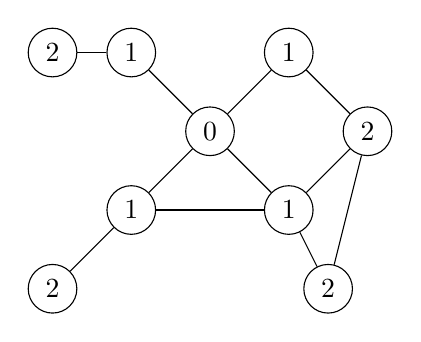
\begin{tikzpicture}[every circle node/.style={draw}]
            \draw (0, 0) node[circle](0){0};
            \draw (1, 1) node[circle](1){1};
            \draw (1, -1) node[circle](2){1};
            \draw (-1, 1) node[circle](3){1};
            \draw (-1, -1) node[circle](4){1};
            \draw (0) -- (1);
            \draw (0) -- (2);
            \draw (0) -- (3);
            \draw (0) -- (4);
            \draw (2) -- (4);
            \draw (-2, 1) node[circle](5){2};
            \draw (3) -- (5);
            \draw (-2, -2) node[circle](6){2};
            \draw (4) -- (6);
            \draw (2, 0) node[circle](7){2};
            \draw (1) -- (7);
            \draw (2) -- (7);
            \draw (1.5, -2) node[circle](8){2};
            \draw (2) -- (8);
            \draw (7) -- (8);
        \end{tikzpicture}    
    \end{center}
    \subsubsection*{Через queue}
    Вершина, в которой начинаем, имеет номер 0, далее заносим в очередь всех её соседей с номером, увеличенным на 1.
    \subsubsection*{0-1 BFS}
    Используется deque, если у вершины номер $x$, то заносим его в начало, если номер $x + 1$, то заносим в конец.
    \subsection{DFS}
    Храним массив посещённых вершин
    \begin{lstlisting}
used[v];
    \end{lstlisting}
    \begin{center}
        Ориентированный:\\
        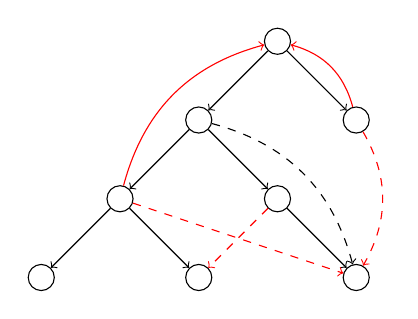
\begin{tikzpicture}[every circle node/.style={draw}]
            \draw (0, 0) node[circle](0){};
            \draw (-1, -1) node[circle](1){};
            \draw (1, -1) node[circle](2){};
            \draw (-2, -2) node[circle](3){};
            \draw (0, -2) node[circle](4){};
            \draw (-3, -3) node[circle](5){};
            \draw (-1, -3) node[circle](6){};
            \draw (1, -3) node[circle](7){};
            \draw[->] (0) -- (1);
            \draw[->] (0) -- (2);
            \draw[->] (1) -- (3);
            \draw[->] (1) -- (4);
            \draw[->] (3) -- (5);
            \draw[->] (3) -- (6);
            \draw[->] (4) -- (7);
            \draw[->, red] (3) to[bend left] (0);
            \draw[->, red] (2) to[bend right] (0);
            \draw[dashed, ->] (1) to[bend left] (7);
            \draw[red, dashed, ->] (3) -- (7);
            \draw[red, dashed, ->] (4) -- (6);
            \draw[red, dashed, ->] (2) to[bend left] (7);
        \end{tikzpicture}\\
        \textit{Термины}: \begin{tikzpicture}
            \draw[->] (0, -0.3) -- node[anchor=south]{ребро обхода} (3, -0.3);
        \end{tikzpicture}, \begin{tikzpicture}
            \draw[dashed, ->] (0, 0) -- node[anchor=south]{прямое ребро} (3, 0);
        \end{tikzpicture}, \begin{tikzpicture}
            \draw[red, ->] (0, 0) -- node[anchor=south, black]{обратное ребро} (3, 0);
        \end{tikzpicture}, \begin{tikzpicture}
            \draw[dashed, red, ->] (0, 0) -- node[anchor=south, black]{перекрёстное ребро} (3.4, 0);
        \end{tikzpicture}
    \end{center}
    \begin{center}
        Неориентированный граф:\\
        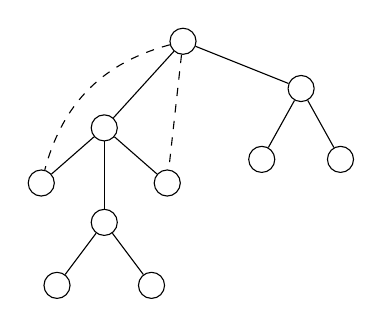
\begin{tikzpicture}[every circle node/.style={draw}]
            \draw (0, 0) node[circle](0){};
            \draw (-1, -1.1) node[circle](1){};
            \draw (0) -- (1); 
            \draw (1.5, -0.6) node[circle](2){};
            \draw (0) -- (2);
            \draw (1, -1.5) node[circle](3){};
            \draw (2) -- (3);
            \draw (2, -1.5) node[circle](4){};
            \draw (2) -- (4);
            \draw (-1.8, -1.8) node[circle](5){};
            \draw (1) -- (5);
            \draw[dashed] (0) to[bend right] (5);
            \draw (-0.2, -1.8) node[circle](6){};
            \draw (1) -- (6);
            \draw[dashed] (0) -- (6);
            \draw (-1, -2.3) node[circle](7){};
            \draw (1) -- (7);
            \draw (-1.6, -3.1) node[circle](8){};
            \draw (7) -- (8);
            \draw (-0.4, -3.1) node[circle](9){};
            \draw (7) -- (9);
        \end{tikzpicture}
    \end{center}
    Не имеет перекрётсных рёбер.\\
    Напишем реализацию DFS с глобальным графом $g$.
    \begin{lstlisting}
void dfs(int vertex_idx) {
    used[vertex_idx] = 1;
    for (auto dest_idx : g[vertex_idx]) {
        if (!used[dest_idx]) {
            dfs(dest_idx);
        }
    }
}
    \end{lstlisting}
    \begin{center}
        Примеры задач на dfs:
    \end{center}
    \begin{enumerate}
        \item Подсчёт количества компонент связности. (В цикле запускаем dfs от всех вершин. Количество запусков dfs совпадёт с количеством компонент связности)
        \item Серия запусков dfs.
        \item Поиск остовного леса.
        \item Двудольность.
        \item Поиск цикла.
        \item Поиск Эйлерова пути (поиск пути, проходящего все рёбра один раз).
    \end{enumerate}
    \begin{center}
        \underline{Обход дерева}
    \end{center}
    Вместо used[v] храним parent[v]. То есть храним предков.\\
    ДП снизу: size[v];\\
    ДП сверху: dep[v];
    \begin{center}
        Лекция 12 ноября
    \end{center}
    \subsection{Приливания}
    Не путать с переливаниями и т.д.\\
    Предположим мы реализуем динамическое программирование на дереве (далее будем называть \textit{динамикой на дереве}).\\
    Пусть нам дано несбалансированное дерево (sz$_i$ --- какая-то метрика поддерева):
    \[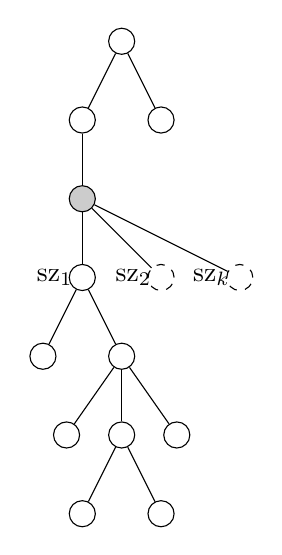
\begin{tikzpicture}
        \draw (-0.5, 0) node(0)[circle, draw]{};
        \draw (-1, -1) node(1)[circle, draw]{};
        \draw (0, -1) node(2)[circle, draw]{};
        \draw (-1, -2) node(3)[circle, draw, fill=gray!40]{};
        \draw (-1, -3) node(4)[circle, draw]{} node[anchor=east]{sz$_{1}$};
        \draw (-1.5, -4) node(5)[circle, draw]{};
        \draw (-0.5, -4) node(6)[circle, draw]{};
        \draw (0) -- (1);
        \draw (0) -- (2);
        \draw (1) -- (3);

        \draw (0, -3) node(12)[circle, dashed, draw]{} node[anchor=east]{sz$_2$};
        \draw (3) -- (12);
        \draw (1, -3) node(13)[circle, dashed, draw]{} node[anchor=east]{sz$_k$};
        \draw (3) -- (13);

        \draw (3) -- (4);
        \draw (4) -- (5);
        \draw (4) -- (6);
        \draw (-1.2, -5) node(7)[circle, draw]{};
        \draw (-0.5, -5) node(8)[circle, draw]{};
        \draw (0.2, -5) node(9)[circle, draw]{};
        \draw (6) -- (7);
        \draw (6) -- (8);
        \draw (6) -- (9);
        \draw (-1, -6) node(10)[circle, draw]{};
        \draw (0, -6) node(11)[circle, draw]{};
        \draw (8) -- (10);
        \draw (8) -- (11);
    \end{tikzpicture}\]
    В сбалансированном дереве может быть sz$_1 > $ sz$_2 > \dots$ sz$_k$\\
    $\forall i \in [2,\ k]$ с конца приливаем sz$_i$ к sz$_{i - 1}$ (приливаем из меньшего в большее), при необходимости добавляем какую-то константу.
    \subsection*{Утверждение}
    В таком случае произойдёт $O(n\log n)$ добавлений.
    \subsection*{Доказательство}
    Возьмём произвольный элемент $x$, пусть у него sz\,$= 1$. Тогда после приливания к следующему элементу, полученный sz будет не менее $2$, далее --- не менее $4$, и т.д. Постоянно получаем sz не менее чем в два раза больше, пока не получим $n$. Тогда будет сделано $O(\log n)$ приливаний.
    \subsection{СНМ (DSU)}
    Расшифровка: ``система непересекающихся множеств''
    $n$ покрашенных элементов, $m$ запросов вида:
    \begin{itemize}
        \item unite($a,\ b$). Присваиваем множествам $a,\ b$ одинаковый цвет.
        \item col($a$). Получить цвет множества.
        \item col($a$)\,$\overset{?}{=}$\,col($b$). Сравниваем цвета множеств.
        \item sz($a$). Размер множества, содержащего элемент $a$.
    \end{itemize}
    \subsubsection*{Наивное решение}
    Хотим иметь col[$a$] --- массив цветов.\\
    Старт: заполняем col[$i$] = color$_i$, заполняем массив sz[color].\\
    unite($a,\ b$):\\
    Пусть ca = col[$a$], cb = col[$b$]. Базовая реализация такого алгоритма:
    \begin{lstlisting}
for (int i = 0; i < n; i++) {
    if (col[i] == ca) {
        col[i] = cb;
        sz[cb]++;
    }
}
    \end{lstlisting}
    Работает за $O(n^2 + m)$.\\
    \subsubsection*{Возможное улучшение (приливания)}
    Для каждого цвета храним (допустим в векторе ind[color]) позиции с элементами этого цвета.\\
    Положим col[$a$]\,$\neq$\,col[$b$]. Тогда нужно сравнить $\underset{\text{num a}}{\underbrace{\text{ind[col[$a$]].size()}}}$ и $\underset{\text{num b}}{\underbrace{\text{ind[col[$b$]].size()}}}$.\\
    Положим num a\,>\,num b больше, тогда 
    \begin{enumerate}
        \item все элементы col[$b$] красим в цвет col[$a$] за $O(\text{num b})$.
        \item В ind[col[$a$]] добавим все индексы из ind[col[$b$]] за $O(\text{num b})$.
    \end{enumerate}
    Всего получим $O(n\log n)$ операция (асимптотика приливаний). Приливаем меньшую часть (её размер не более $\frac{1}{2^{k + 1}}$, где $k$ --- количество совершённых операций unite) к большей.
    \subsubsection*{Возможное улучшение (лес)}
    Храним массив предков каждой вершины (предком корня является корень). Изначально каждую вершину считаем корнем дерева, содержащего только эту вершину. Далее все вершины, попавшие в поддерево какой-то вершины считаются покрашенными в цвет корня.\\
    Старт: массив parent[$i$] = $i$.\\
    Цвет --- номер корня дерева.\\
    unite($a,\ b$): $\left.\begin{matrix}
        a = \text{col($a$)}\\
        b = \text{col($b$)}
    \end{matrix}\right\}\rightarrow a\neq b\Rightarrow$ подвешиваем ``меньшего'' к ``большему''.\\
    Сравнивать вершины можно
    \begin{itemize}
        \item[-] По высоте
        \item[-] По размеру 
    \end{itemize}
    Работает за $O(n\log n + m\log n)$ первое слагаемое --- выполнение всех операций unite, второе --- поиск предка (цвета) вершины.
    \subsubsection*{Эвристика сжатия пути}
    Пусть дано дерево:
    \[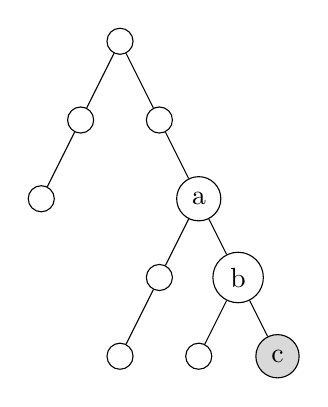
\begin{tikzpicture}[every circle node/.style={draw}]
        \draw (0, 0) node(0)[circle]{};
        \draw (-0.5, -1) node(1)[circle]{};
        \draw (-1, -2) node(2)[circle]{};
        \draw (0) -- (1);
        \draw (1) -- (2);
        \draw (0.5, -1) node(3)[circle]{};
        \draw (0) -- (3);
        \draw (1, -2) node(4)[circle]{a};
        \draw (0, -4) node(9)[circle]{};
        \draw (3) -- (4);
        \draw (1.5, -3) node(5)[circle]{b};
        \draw(4) -- (5);
        \draw (0.5, -3) node(6)[circle]{};
        \draw (6) -- (9);
        \draw (4) -- (6);
        \draw (1, -4) node(7)[circle]{};
        \draw (2, -4) node(8)[circle, fill=gray!30]{c};
        \draw (5) -- (7);
        \draw (5) -- (8);
    \end{tikzpicture}\]
    Пусть мы хотим узнать цвет вершины c, тогда дерево перейдёт:
    \[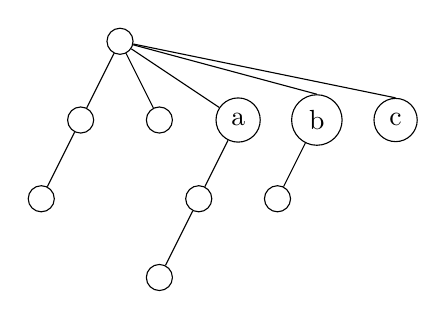
\begin{tikzpicture}[every circle node/.style={draw}]
        \draw (0, 0) node(0)[circle]{};
        \draw (-0.5, -1) node(1)[circle]{};
        \draw (-1, -2) node(2)[circle]{};
        \draw (0) -- (1);
        \draw (1) -- (2);
        \draw (0.5, -1) node(3)[circle]{};
        \draw (0) -- (3);
        \draw (1.5, -1) node(4)[circle]{a};
        \draw (0.5, -3) node(9)[circle]{};
        \draw (0) -- (4);
        \draw (2.5, -1) node(5)[circle]{b};
        \draw (0) to[] (5.north);
        \draw (1, -2) node(6)[circle]{};
        \draw (4) -- (6);
        \draw (6) -- (9);
        \draw (2, -2) node(7)[circle]{};
        \draw (3.5, -1) node(8)[circle]{c};
        \draw (5) -- (7);
        \draw (0) to[] (8.north);
    \end{tikzpicture}\]
    Это \cancel{честно честно} работает за $O(\alpha(n)\cdot n + m)$. $\alpha(n)$ --- некая функция (обратная функции Аккермана), которая во всех реальных задачах не более $4$.
    \subsection*{СНМ с откатами}
    Операции:
    \begin{itemize}
        \item[-] unite($a,\ b$)
        \item[-] $a\sim b$
        \item[-] sz[$a$]
        \item[-] rollback()
    \end{itemize}
    \textbf{Не делаем сжатие}
\end{document} 